% !TEX program = pdflatex
\documentclass[11pt]{article}
\usepackage[margin=0.72in]{geometry}
\usepackage[T1]{fontenc}
\usepackage[utf8]{inputenc}
\usepackage{lmodern,microtype,parskip,enumitem,fancyhdr,setspace,needspace,graphicx,float}
\usepackage[table]{xcolor}
\usepackage{hyperref,tcolorbox}
\definecolor{PrimaryRed}{HTML}{8B1E1E}
\definecolor{DeepNavy}{HTML}{15324A}
\definecolor{Addition}{HTML}{164F78}
\definecolor{SoftBlue}{HTML}{E7F0F6}
\hypersetup{colorlinks=true,urlcolor=DeepNavy,linkcolor=DeepNavy,pdftitle={Invisible Invaders},pdfauthor={Piter Zacari Garcia Bautista}}
\setlength{\parindent}{0pt}\setlength{\parskip}{0.36em}\setstretch{1.02}
\newcommand{\secx}[1]{\par\Needspace{5\baselineskip}\addvspace{0.10in}{\Large\bfseries\color{PrimaryRed}#1}\par\color{DeepNavy}\hrule\color{black}\vspace{0.08in}}
\newcommand{\original}[1]{{\color{black}#1}}
\newcommand{\revision}[1]{{\color{Addition}\textbf{REVISION:} #1}}
\newtcolorbox{focusbox}{colback=SoftBlue,colframe=DeepNavy,boxrule=0.6pt,arc=2pt,left=7pt,right=7pt,top=6pt,bottom=6pt}
\begin{document}
\begin{titlepage}\thispagestyle{empty}\begin{center}
{\large University of Rochester\\ Warner School of Education}\\[0.18in]
{\color{PrimaryRed}\rule{\textwidth}{1.5pt}}\\[0.2in]
{\Huge\bfseries Invisible Invaders}\\[0.15in]
{\LARGE Youth, Evidence, and Environmental Justice}\\[0.17in]
{\Large EDE477 --- Science Major Project}\\[0.15in]
\vfill\begin{focusbox}\centering\textbf{Guiding question}\\ How can tiny fragments move through our environment, and how can we investigate and respond fairly?\end{focusbox}\vfill
\begin{tabular}{rl}\textbf{Student} & Piter Zacari Garcia Bautista \\
\textbf{Course} & Teaching and Learning in the Content Areas \\
\textbf{Instructor} & Amy Stell \\
\textbf{Foundation} & Get Real! Science Camp --- Invisible Invaders\end{tabular}\vfill
{\itshape Young people are investigators, model builders, and partners in change.}\par
{\color{PrimaryRed}\rule{5in}{0.8pt}}\end{center}\end{titlepage}
\pagestyle{fancy}\fancyhf{}\lhead{\small Piter Garcia}\rhead{\small EDE477 --- Invisible Invaders}\cfoot{\thepage}\setlength{\headheight}{14pt}
\secx{Original Activity and Purpose}
\textbf{Source.} This revision builds on the July 27, 2026 \href{https://docs.google.com/document/d/1jc_dSOKXVhSoSbvfbivXlgfYOxrrJ2L6KwbR7LQZCLc/edit}{Invisible Invaders Monday lesson}, co-planned and co-facilitated by Piter Garcia and Aastha in Get Real! Science Camp, and our post-camp implementation revision. The \textit{Monday Lesson: How Small? How Does It Move?} is the primary activity; this journal reproduces selected original language, and Appendix A includes the complete original Activity 2 text (the scale-and-wind investigation) in black. It proposes a focused redesign of that investigation and its supporting model-building sequence; the broader Monday lesson remains accessible at the source link. The original is not attributed to me alone.

\textbf{Reading key:} \original{black = original source text (complete for Activity 2 in Appendix A, with selected original/base passages in the main sequence)}; \revision{blue = proposed additions and changes.} The written labels also distinguish the versions in grayscale. The original already contains justice and access supports; the redesign extends those strengths using later youth feedback and EDE477 readings.

\begin{focusbox}\original{\textbf{Original student-facing question:} How small can plastic pieces get, how can moving air or water carry them, and what do we still not know?}\\[4pt]
\original{\textbf{Original Gotta-Have 2 --- WATER:} Water transports materials.}\end{focusbox}

\original{\textbf{Original Monday success:} Youth use Friday's observations, Aastha's scale and wind investigations, and one short source to begin a first-draft before $\rightarrow$ during $\rightarrow$ after model. Every idea or question may enter the draft. Monday is for making thinking visible, not completing the week-long explanation or grading ideas as right or wrong.}

\revision{Invite students to begin with a locally meaningful observation, question, or example they choose. Preserve the original question as a possible starting point, then let the group decide what a model or investigation should help explain. Share the reason for each next activity: notice a puzzle $\rightarrow$ test a mechanism $\rightarrow$ revise an explanation $\rightarrow$ consider a fair response. No personal or family disclosure is required.}

\secx{Revised Investigation}
\revision{\textbf{Storyline launch --- students' evidence stories:} Before introducing the scale tools, invite each scholar to choose a Friday sampling photo, observation, method, or question and tell the evidence story in their own way: orally, by drawing or pointing, with a partner, through selected labels, or by passing and returning. Ask what the group still needs to explain and let that question motivate the scale and transport tests. After the model revision, return to the original story and ask what changed, what remained uncertain, and whose questions need to shape the next investigation. No personal or family disclosure is required.}
\subsection*{1. Scale: What can our tools show?}
\original{Show or measure 1 meter, 10 centimeters, 1 centimeter, 5 millimeters, and 1 millimeter. Ask scholars to choose measuring, holding, cutting, labeling, checking, observing, or pass-and-return roles.}

\revision{Show the entire visual sequence while giving one direction at a time. Offer large-print and tactile measurement markers, shared manipulation, pointing, partner narration, or a seated observation route. Invite students to test the claim ``All microplastics are invisible'' using an appropriate source and the scale tools. Keep their initial reasoning visible and ask what the tools cannot resolve. Some microplastics are visible; small size alone does not identify a particle's material. Avoid timed competition and permit breaks or re-entry without penalty.}

\subsection*{2. Transport: What happens when air moves?}
\original{Place exactly 12 lightweight paper pieces inside the same taped starting box and mark one finish line. ``These paper pieces are a model for lightweight fragments. Move at least half across the boundary without touching them with your hands.''}

\original{Record the starting count, how many pieces crossed the finish line, the direction they moved, and where pieces stopped. Count pieces that did not move too.}

\revision{Students decide a question such as how fan distance or paper shape might affect movement, then choose one feasible comparison with the teacher. Record what is changed, what is kept similar, and the results for all pieces. Students may fan, observe, count, draw, photograph materials, dictate, or work with a partner; breathing is not required. Paper is a \emph{proxy}, not collected microplastic. Its movement illustrates a possible transport mechanism and cannot establish what happened at a particular site. Ask what a water-transport investigation would need to change.}

\subsection*{3. From observation to a revisable model}
\original{BEFORE --- SOURCE + RELEASE: What product or material contained plastic? How could smaller pieces or fibers leave it? DURING --- MOVE + ENCOUNTER: How could air, water, soil, or food transport it? What living thing might encounter it? AFTER --- EVIDENCE + UNKNOWN + FAIR ACTION: What supports an arrow? What remains possible or unknown? Who can reduce the pathway or share responsibility?}

\revision{First, individuals or small groups create an initial before/during/after explanation. They can use drawing, movable labels, oral recording, writing, or a combination. Label each arrow \emph{observation}, \emph{possible pathway}, or \emph{question}. Next, each group selects an observation and explains what it supports and what it cannot establish. Peers offer an addition, a reasoned revision, or a question; the model creators decide how to respond. Preserve an initial and revised version so the change in reasoning remains visible. A shared model follows without requiring every group to erase uncertainty.}

\begin{figure}[H]\centering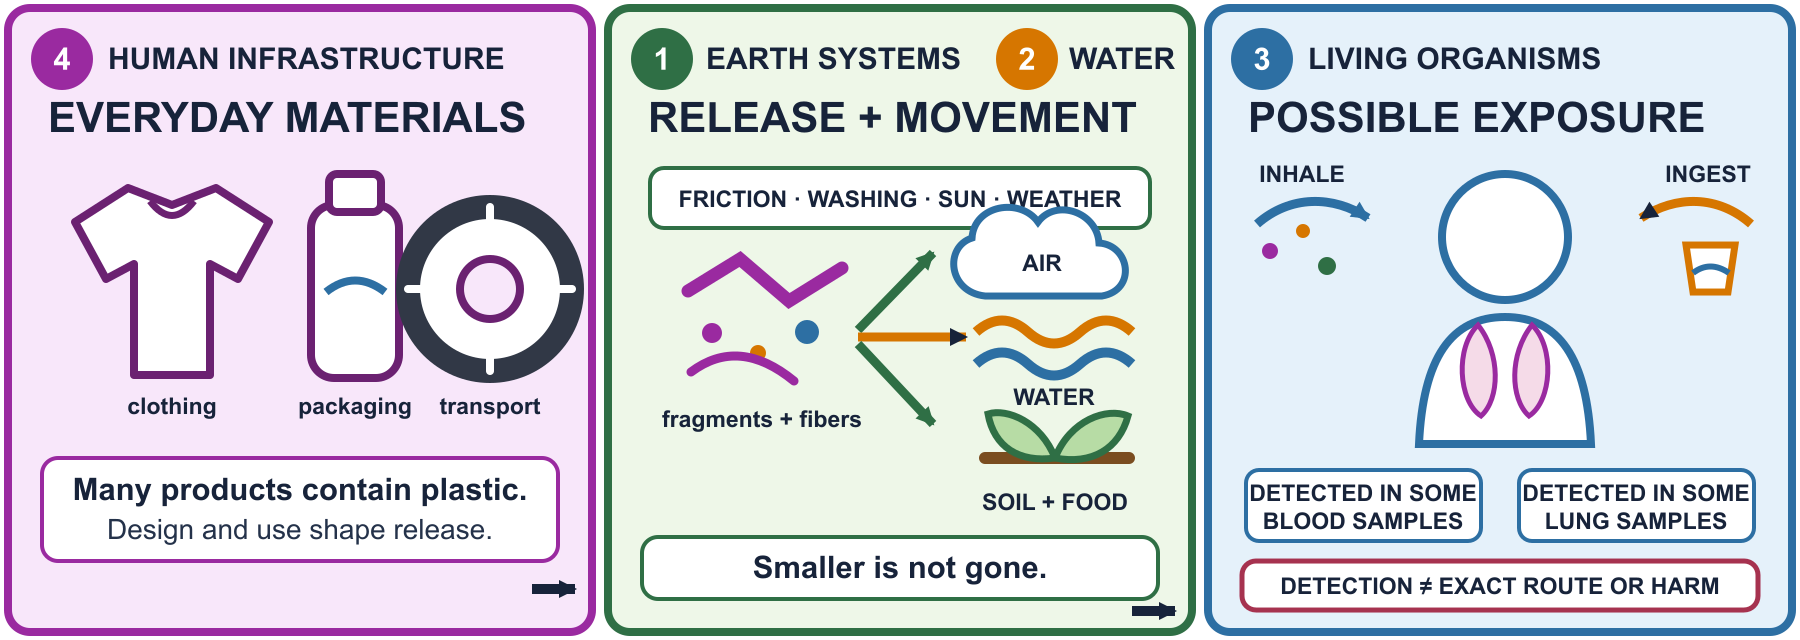
\includegraphics[width=0.98\textwidth]{figures/camp-model.png}\caption{Existing Invisible Invaders sample model: products, release and movement, and possible exposure. This is an instructional representation, not a youth result or proof of a specific exposure pathway. Detection in a sample does not establish an exact route or a health effect.}\label{fig:model}\end{figure}

\subsection*{4. Field evidence and fair action}
\original{Begin with youth thinking from Friday. Do not begin by announcing the pathway. Give the challenge, wait, then follow up. Let scholars try, revise, and make mistakes before offering a hint.}

\revision{If an approved field investigation is available, revisit the sample labels and site records using the same method at each chosen site. Figure~\ref{fig:sampling} provides the original visual sequence; teachers check site rules and current local procedures before use. Keep samples separate. A suspected particle is not confirmed plastic without appropriate identification. Ask whose questions and knowledge shape the inquiry, who bears responsibility for sources and infrastructure, and who should participate in decisions. Students choose a realistic response, such as a question for a local organization, a public explanation, or a proposal that considers producers and infrastructure as well as individual actions. No student must reveal a home location.}

\begin{figure}[H]\centering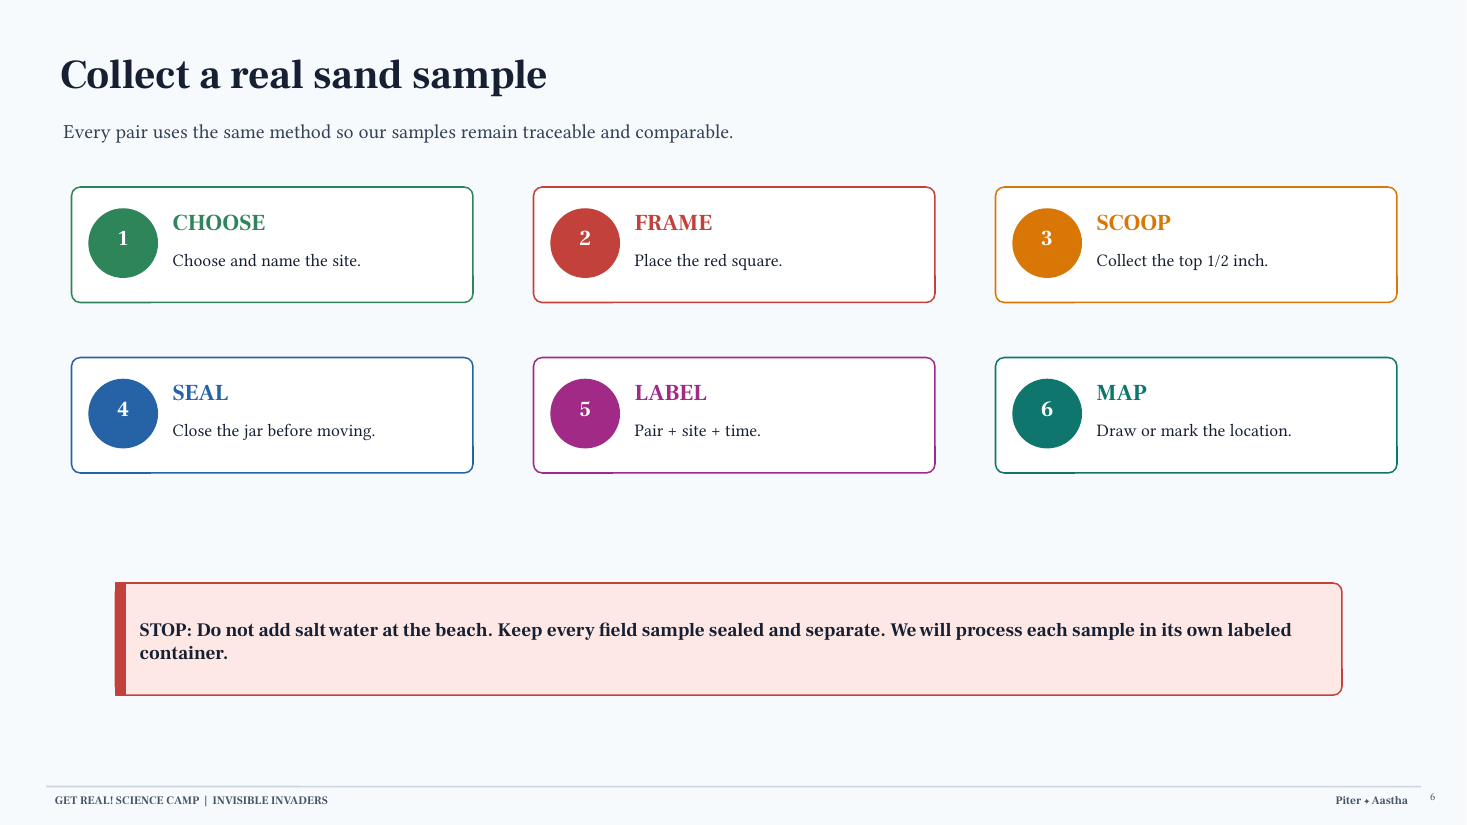
\includegraphics[width=0.91\textwidth]{figures/sampling-steps.png}\caption{Existing camp sampling visual: choose, frame, scoop, seal, label, and map. The sequence supports traceability; the samples alone do not establish material identity, exposure, or harm.}\label{fig:sampling}\end{figure}

\subsection*{5. Access and evidence in assessment}
\revision{Use a common evidence standard across expression modes: each student identifies an observation, proposes and explains one relationship, distinguishes what remains unknown, and describes what evidence could revise the model. Offer a visual agenda, captions, time to process, alternative sensory routes, and a choice to pass and return. These are options, not assumptions about what any particular learner needs. Ask students how the supports worked and adapt them. If extending to fish-related evidence, preview the sensory demands, offer an equivalent non-fish route, and keep chemical handling adult-only.}

\newpage
\secx{Reflective Justification}
Co-facilitating Invisible Invaders with Aastha gave me a concrete way to connect scientific thinking with the questions young people bring to a place. Our camp record describes youth sampling, using a moving-air model, revising shared explanations, and considering community action. It also records requests for more time to build and investigate, less rushing, more movement, and a sensory-safe alternative to the fish activity (Garcia \& Aastha, 2026). I treat those requests as guidance for the next design, not as proof that any one support worked for everyone.

I chose the camp lesson because its before/during/after model already joins science with student questions. I want to make the connection between each activity and the developing explanation even clearer. Reiser et al. (2021, pp.~811--812, 818--820) describe a storyline in which learners can see why the next investigation follows from what they have figured out. Here, the scale challenge and paper-transport test each provide a reason to revisit a specific model arrow. Students then decide what to investigate or communicate next instead of completing isolated stations.

The redesign also makes uncertainty a part of doing science. Krajcik and Merritt (2012, pp.~10--13) describe models as simplified representations that students develop and revise against evidence. Windschitl and Thompson (2013, pp.~65--68) use peer questions and explanations to make that revision visible. Paper moving in air can suggest a mechanism; a suspected particle is not automatically confirmed plastic. Neither observation proves an exposure route or health effect. I want students to be able to name both what they learned and the next evidence they need.

JuST asks whose knowledge shapes the investigation and how science can support meaningful action. Luehmann et al. (2024, pp.~334--340, 347--350) connect local experiences and multilingual expertise with inquiry and community action. I extend that orientation by asking students to examine responsibility across product design, infrastructure, monitoring, and policy, without assigning a predetermined answer. Our EDE477 water investigation reinforces the same need to keep a result distinct from a claim about cause or safety.

My Puzzle Plan/EQUITAS lens connects this work to overlapping identities and access. Language, culture, migration, neurodivergence, disability, health, and prior experiences may shape participation together. In my teaching, a quiet, seated, visual, partner-supported, or delayed response can make reasoning available without lowering the expectation for evidence. Our post-camp reflection reminds me to invite feedback and change the design rather than infer a learner's needs from a label. I want students to see themselves as people whose questions and explanations can shape science and fair action.

\newpage\secx{References and Source Notes}
Garcia, P., \& Aastha. (2026). \textit{Invisible Invaders: Post-camp implementation revision addendum}. EDU486 camp work. The related Monday lesson, linked below, was co-planned.

\href{https://docs.google.com/document/d/1jc_dSOKXVhSoSbvfbivXlgfYOxrrJ2L6KwbR7LQZCLc/edit}{Invisible Invaders Monday lesson and activity sequence}. (2026). Get Real! Science Camp. Figure~\ref{fig:model} and Figure~\ref{fig:sampling} are existing camp instructional visuals; their labels and scientific limitations are preserved.

Krajcik, J., \& Merritt, J. (2012). Engaging students in scientific practices: What does constructing and revising models look like in the science classroom? \textit{Science and Children}, 10--13.

Luehmann, A., Zhang, Y., Boyle, H., Tulbert, E., Merliss, G., \& Sullivan, K. (2024). Toward a justice-centered ambitious teaching framework: Shaping ambitious science teaching to be culturally sustaining and productive in a rural context. \textit{Journal of Research in Science Teaching, 61}, 319--357. \url{https://doi.org/10.1002/tea.21917}

Reiser, B. J., Novak, M., McGill, T. A. W., \& Penuel, W. R. (2021). Storyline units: An instructional model to support coherence from the students' perspective. \textit{Journal of Science Teacher Education, 32}(7), 805--829. \url{https://doi.org/10.1080/1046560X.2021.1884784}

Windschitl, M., \& Thompson, J. J. (2013). The modeling toolkit: Making student thinking visible with public representations. \textit{The Science Teacher}, 63--69.

\textit{Water Test Investigation}. (2026). Collaborative EDE477 course activity. \url{https://docs.google.com/document/d/1GpqZl8MVNCpH4dKFZKeCQcLOGir0535jPK4ayxFyxEs/edit}

\textbf{Process disclosure.} OpenAI Codex assisted in organizing the co-facilitated camp lesson, post-camp record, EDE477 readings, existing instructional visuals, and Piter's stated priorities into this LaTeX revision. Source passages are labeled, and proposed changes are identified separately. The source camp documents and team attribution remain intact.

\newpage\secx{Appendix A --- Complete Original Lab/Activity Text}
\textit{Source: Activity 2, \emph{Impossible Cut + Escape the Wind + watch and wonder}, from the co-planned July 27, 2026 \href{https://docs.google.com/document/d/1jc_dSOKXVhSoSbvfbivXlgfYOxrrJ2L6KwbR7LQZCLc/edit}{Invisible Invaders Monday lesson}. The same lesson is available free in the \href{https://github.com/pzg8794/EDU486/blob/main/assignments/03-camp-unit-plan/monday-water-pathways-and-first-model.md}{public EDU486 archive}. Source wording and sequence are reproduced below, not reinterpreted; black indicates original text. The blue revisions elsewhere are proposed changes, not claimed as previously implemented.}\par\medskip
\begingroup\small
\textbf{Activity 2 - Impossible Cut + Escape the Wind + watch and wonder (9:32-10:10)}\par
\noindent\original{AA gives the Impossible Cut challenge first and lets everyone, including Piter, try before offering measuring steps or hints. Compare 1 m, 10 cm, 1 cm, 5 mm, 1 mm, and 1 micrometer, then ask what classroom tools can and cannot make or verify. Show the intentionally inaccurate claim ``All microplastics are invisible.'' Place AGREE / NOT SURE / DISAGREE placards along a continuum from strongly agree to strongly disagree. Standing or moving is one route; pointing to or holding a placard while seated, asking a partner to place a marker, or passing and returning are equally valid. Name needed evidence and revise after the scale source: some microplastics are visible and others require magnification. The false sentence is a claim to test, not an answer to copy.}\par\medskip
\noindent\original{AA then leads Escape the Wind (see Monday teaching slides, Moving-Air Transport Model) with exactly 12 paper proxies inside one taped starting box and one finish line. Without touching the pieces, scholars choose cardboard, a clipboard, notebook, or paper fan and try to move them. Give each person one equal-length turn. Breath is optional, never required. Name the paper as a transport model, not microplastic evidence.}\par\medskip
\noindent\original{By 10:00, record the 12-piece starting count, how many crossed the finish line, the direction moved, where pieces stopped, and pieces that did not move. This is the transport pattern. Count all 12 pieces during cleanup. Scholars choose one vetted short video together, then speak, write, draw, point, dictate, or pass. Scholars may record their own exact Wonder Wall questions; AA or PG offers to scribe only when wanted.}\par\medskip
\noindent\original{Protect the 10:10-10:20 snack, movement, seated, or quiet reset.}\par\medskip
\noindent\original{Evidence of success: scholars explain that smaller scales may require different tools, moving air transported the paper model, and neither classroom model proves that a particle is plastic or establishes every environmental route.}\par\medskip
\noindent\original{Keep the Friday souvenir, scale sequence, and Wonder Wall visible through the break. Preview: ``Next Piter will help us combine our evidence and questions into one model.''}\par\medskip
\noindent\original{``Our cut paper and wind activity are models: each shows some things and leaves others out. A globe can show relative locations but not stars or exact travel distances. After the break, we will collect every scholar idea and question without judging it right or wrong; we can revise during the week.''}\par\medskip
\noindent\original{Puzzle piece: [SCIENCE + EVIDENCE + JUSTICE/ACTION] Combine Friday's two places, the scale and transport models, one short source, and youth questions in a power-aware before/during/after consensus model.}\par\medskip
\noindent\original{PICRAT: Interactive / Transform}\par\medskip
\endgroup
\end{document}
